\chapter{Máquinas CNC}

Las máquinas automatizadas de fabricación digital o CNCs son sistemas mecatrónicos programables que ejecutan procesos de manufactura mediante un set de instrucciones definido en un programa. Incluyen tecnologías como la impresión 3D, torneado, fresado, corte láser y robots industriales. Se caracterizan por su precisión, repetibilidad y autonomía operativa, lo que les permite fabricar piezas diversas y complejas de manera sencilla.

\section{Flujo del proceso de fabricación digital}

Las tecnologías de fabricación digital se fundamentan en un proceso computarizado que abarca desde el diseño hasta la producción de la pieza final (Figura \ref{digfab}). Este proceso comienza con la modelación de la componente deseada mediante un software de diseño asistido por computadora (CAD, Computer-Aided Design). Este tipo de herramientas no solo permite crear y visualizar el modelo tridimensional de la pieza, sino también analizar su integración dentro de un sistema ensamblado y evaluar su desempeño mecánico mediante técnicas como el análisis por elementos finitos (FEA, Finite Element Analysis).

\begin{figure}[h!]
    \centering
    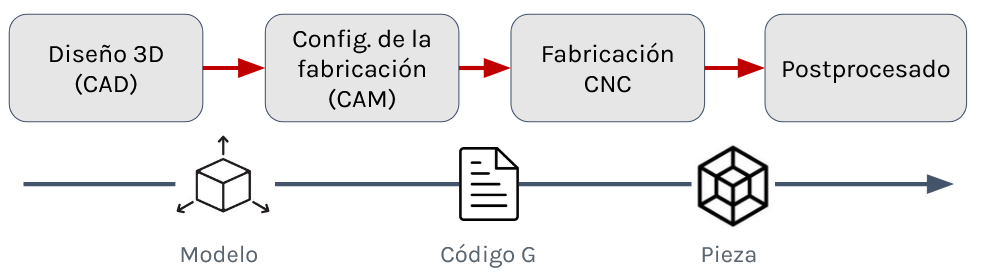
\includegraphics[width=0.9\linewidth]{imgs/digfab.png}
    \caption{Flujo de trabajo para un proceso de fabricación digital.}
    \label{digfab}
\end{figure}

Una vez completado el modelo CAD, este se exporta en un formato de archivo compatible con el software de manufactura asistida por computadora (CAM, Computer-Aided Manufacturing), el cual es específico según el tipo de proceso de fabricación. En el entorno CAM se configuran los parámetros clave del proceso, como velocidades de corte, trayectorias de herramientas y condiciones de operación, con el objetivo de optimizar variables críticas como la calidad del producto final, los costos de producción y el tiempo de fabricación. Además, el software permite simular virtualmente el proceso para verificar su viabilidad, asegurar la compatibilidad con la máquina seleccionada y anticipar posibles errores. Finalmente, el sistema CAM genera un archivo de instrucciones, comúnmente denominado \textbf{código G}, que actúa como entrada para la máquina de fabricación digital, la cual ejecuta el proceso de manera automatizada.

Una vez ejecutados todos los procesos definidos digitalmente, el flujo de trabajo concluye con la etapa de postprocesamiento. Generalmente, esto implica la remoción de la pieza de la máquina y la realización de operaciones complementarias necesarias para alcanzar las condiciones finales del producto. Estas operaciones pueden incluir tareas como el acabado superficial, la limpieza, o la eliminación de estructuras de soporte. En situaciones donde el control de calidad resulta relevante, también se incorpora una fase de metrología para verificar que la pieza cumpla con las especificaciones dimensionales y funcionales establecidas en el diseño.

\section{Sistema}

Cualquier máquina CNC está compuesta de un conjunto de subsistemas primarios (Figura \ref{cncsis}), los cuales generan una \textbf{arquitectura cinemática} (Figura \ref{kinsfig}) de control bidimensional o tridimensional, y subsistemas secundarios, los cuales son de apoyo o específicos del proceso productivo.

\begin{figure}[h!]
    \centering
    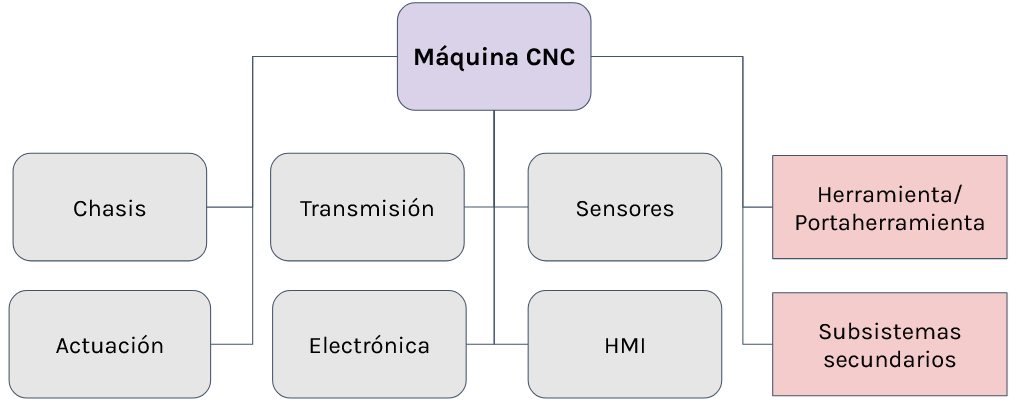
\includegraphics[width=0.9\linewidth]{imgs/cnc.png}
    \caption{Subsistemas en una máquina CNC.}
    \label{cncsis}
\end{figure}

El proceso de fabricación estará determinado por la \textbf{herramienta} o \textbf{portaherramienta} que posea la máquina. Por ejemplo, si se monta un extrusor de plástico la máquina podría funcionar como impresora 3D, y si se cambia por un \textbf{spindle} (portaherramienta rotatorio) la misma máquina podría actuar como fresadora. Si bien, la máquina podría llevar a cabo ambos procesos, la naturaleza de sus subsistemas la hará más idónea para uno de estos.

Entre estos subsistemas primarios se tiene:

\begin{itemize}
    \item \textbf{Interfaz de usuario (HMI):} Permite la comunicación entre el operador y la máquina, para la entrada de comandos, monitoreo de estado y visualización de información relevante. Puede ser una pantalla montada en la máquina, la interfaz de un software o un sistema operativo dedicado.

    \item \textbf{Electrónica:} Incluye al controlador, fuente de poder, y drivers de control de actuadores. Gestiona el procesamiento de señales, comunicación y alimentación. Habitualmente se encuentra como una caja aislada del resto del sistema.

    \item \textbf{Actuadores:} Conjunto de componentes que modifican el estado del sistema, como lo harían motores para el desplazamiento del cabezal en la arquitectura cinemática.

    \item \textbf{Chasis:} Proporciona la estructura mecánica de soporte para el resto de subsistemas. Determina la rigidez, alineamiento y estabilidad durante el funcionamiento de la máquina.

    \item \textbf{Transmisión:} Transfiere el movimiento desde los actuadores hasta los componentes móviles, mediante mecanismos como husillos, correas, engranajes o cremalleras.

    \item \textbf{Sensores/instrumentación:} Capturan información del estado físico de la máquina (posición, temperatura, límites, etc.) para permitir el control del sistema.
\end{itemize}

\begin{figure}[h!]
    \centering
    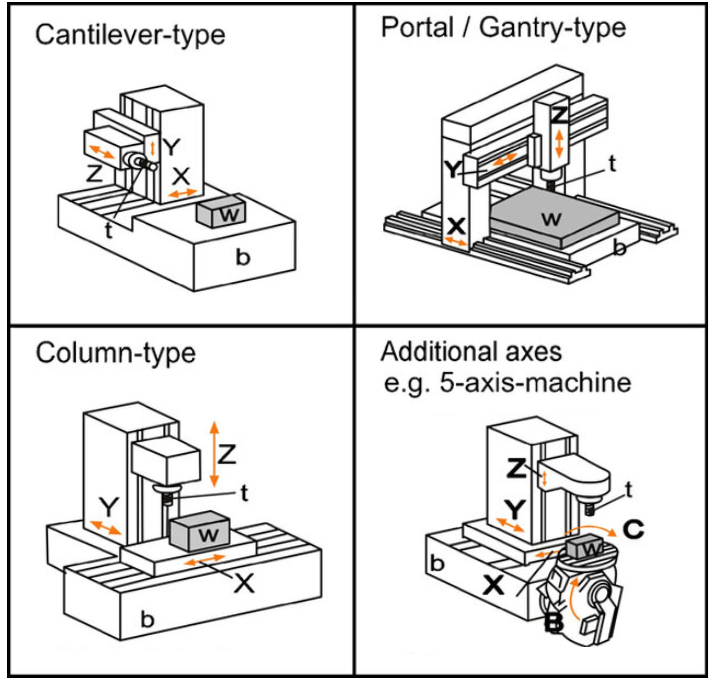
\includegraphics[width=0.67\linewidth]{imgs/kins.png}
    \caption{Ejemplos de arquitecturas cinemáticas.}
    \label{kinsfig}
\end{figure}

\section{Motores stepper}

El control de la posición de un componente o sistema electromecánico suele ser actuado mediante motores eléctricos. La mayoría de los motores eléctricos no otorgan un control directo de la posición de su eje o rotor, sino que es necesario instrumentalizar el sistema con un sensor de tipo \textit{encoder} que mida esta posición y la retroalimente al sistema de control, estableciendo un lazo cerrado (Figura \ref{controlup}). Si bien, esto permitiría un control preciso, el trade-off con la complejidad y costos adquiridos podría no ser conveniente.

\begin{figure}[h!]
    \centering
    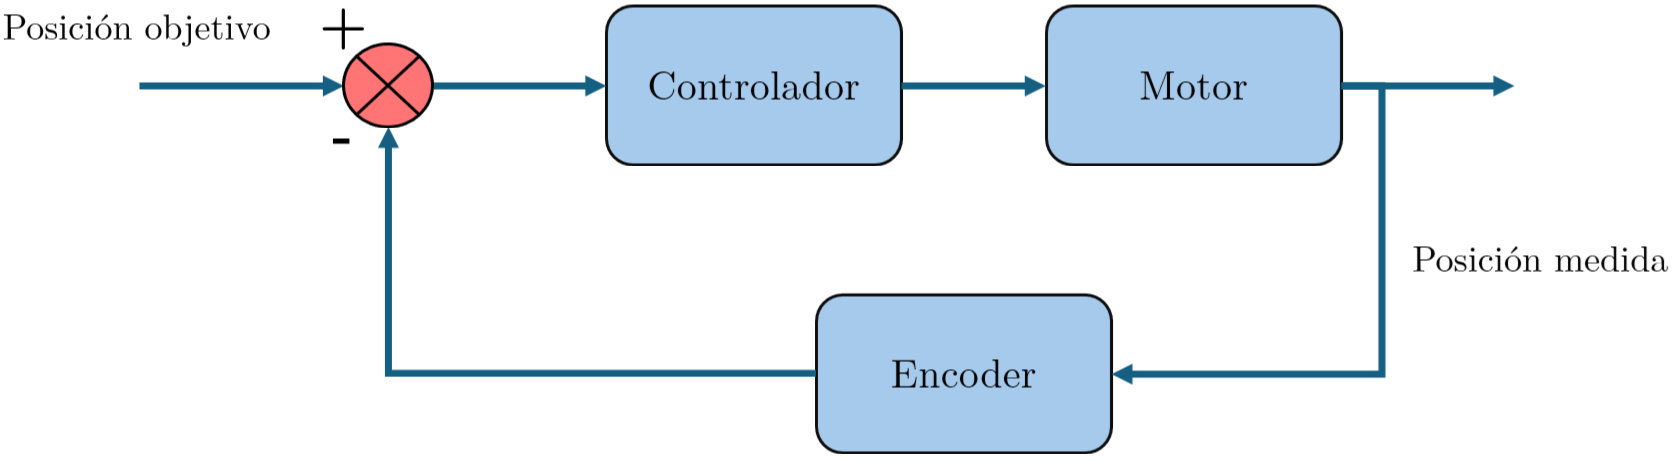
\includegraphics[width=0.9\linewidth]{imgs/controlup.png}
    \caption{Diagrama de control cerrado para controlar la posición de un sistema mediante un motor.}
    \label{controlup}
\end{figure}

Los motores eléctricos de tipo stepper (Figura \ref{stpi}) rotan un arco constante (o un paso, típicamente 1.8$^\circ$) cuando reciben una señal de control. De esta manera, es posible establecer un sistema de control de lazo abierto (sin la parte inferior del loop en la Figura \ref{controlup}) para imponer el perfil cinemático del rotor y la posición final, ofreciendo una opción más sencilla de control. 

\begin{figure}[h!]
    \centering
    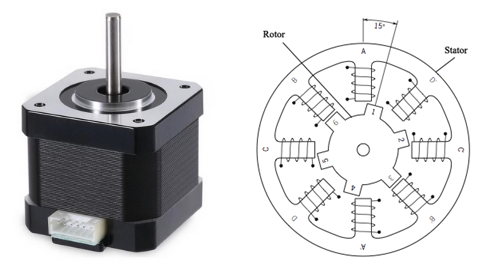
\includegraphics[width=0.7\linewidth]{imgs/stps.png}
    \caption{Motor paso a paso NEMA17 y diagrama de estructura interna.}
    \label{stpi}
\end{figure}

Esto se debe al diseño del motor, en el que el rotor (la parte móvil) está compuesto por un conjunto de imanes permanentes dispuestos de manera intercalada. Estos imanes interactúan con el estator, que consta de bobinas que reciben la señal eléctrica de control. La polarización secuencial de las bobinas genera un campo magnético variable, que provoca el movimiento del rotor, posicionándolo en diferentes puntos de equilibrio. En cada uno de estos puntos, las fuerzas de atracción y repulsión magnéticas se equilibran, permitiendo que el rotor se desplace con precisión o permanezca en una posición fija.

La corriente a través de estas bobinas determinará el torque que puede ejercer el motor contra la carga. En caso de que la carga supere el torque del motor, este no rotará cuando corresponda o se moverá en la dirección opuesta, perdiendo pasos sin que el controlador lo note directamente, induciendo un error en el proceso.

Por lo anterior, versiones más costosas de estos motores incluyen un sistema de sensado, en caso de que la precisión sea crítica o no se trabaje necesariamente en condiciones completamente determinadas.

Los motores paso a paso se clasifican comúnmente según un estándar que define sus dimensiones físicas, particularmente el tamaño de la cara de montaje. Esta clasificación, establecida por la National Electrical Manufacturers Association (NEMA, Figura \ref{nmas}), utiliza números como NEMA 17, NEMA 23, NEMA 34, entre otros, que indican el ancho del marco en décimas de pulgada. Es importante destacar que esta designación solo hace referencia a las dimensiones externas del motor, por lo que dos motores con el mismo número NEMA pueden presentar diferencias significativas en cuanto a torque, corriente nominal, tipo de conexión y otras características eléctricas o mecánicas.

\begin{figure}[h!]
    \centering
    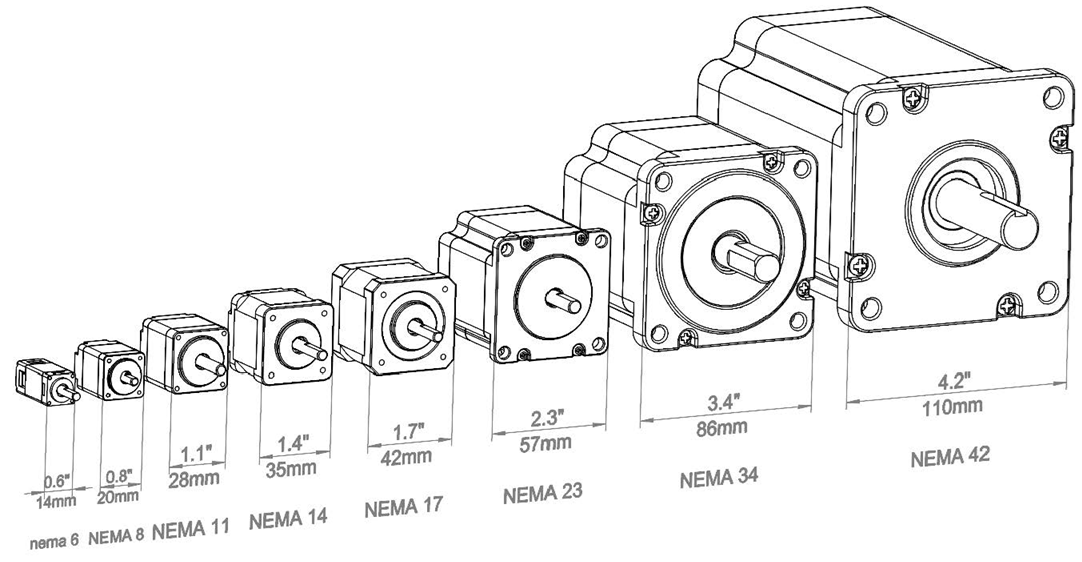
\includegraphics[width=0.9\linewidth]{imgs/nemas.png}
    \caption{Motores paso a paso NEMA.}
    \label{nmas}
\end{figure}

Esta forma de construcción estandarizada brinda flexibilidad al diseño de las máquinas, ya que permite sustituir un motor por otro con las mismas dimensiones de montaje (misma designación NEMA) pero con diferentes especificaciones eléctricas o mecánicas, sin necesidad de realizar modificaciones estructurales, siempre que haya espacio disponible y las condiciones electrónicas lo permitan. Generalmente, los motores NEMA con mayor torque presentan una mayor longitud del cuerpo. Además, existen variantes con diferente ángulo de paso, tipos de eje (plano, estriado, con chavetero), ejes dobles, entre otras configuraciones.

\begin{table}[h]
\centering
\caption{Comparativa estimada de motores paso a paso NEMA. NOTA: Los valores provienen de fabricantes de EEUU, Japón y Alemania, es posible encontrar motores de fabricación China a un tercio del precio pero de prestaciones distintas.}
\label{tab:stepper_nema_comparison}
\begin{tabular}{lccc}
\toprule
\textbf{NEMA} & \textbf{Torque (N·m)} & \textbf{Potencia estimada (W)} & \textbf{Costo aprox. (USD)} \\
\midrule
11 & 0.008 – 0.023 & 1 – 3 & 150 – 170 \\
17 & 0.5 – 0.72 & 10 – 20 & 65 – 95 \\
23 & 0.4 – 3.0 & 20 – 50 & 70 – 130 \\
34 & 4.5 – 12.0 & 50 – 120 & 140 – 220 \\
\bottomrule
\end{tabular}
\end{table}

Mediante la configuración del driver, dispositivo encargado de transformar las señales del controlador en corriente adecuada para las bobinas del motor, es posible ajustar el modo de operación del motor paso a paso, permitiendo dividir cada paso completo en fracciones más pequeñas, como 1/2, 1/4, 1/8, entre otras. Esta técnica, conocida como \textit{microstepping}, permite mejorar la resolución y suavidad del movimiento. No obstante, a medida que se incrementa el nivel de subdivisión, el torque disponible por micro-paso disminuye, debido a que las corrientes aplicadas no alcanzan los valores máximos en cada fase. Por esta razón, si bien el torque total del motor no se reduce, la capacidad de generar fuerza efectiva por paso se ve limitada, especialmente a bajas velocidades.

En una máquina CNC, los motores están físicamente conectados con una transmisión, luego existe una relación entre su desplazamiento rotacional y el de la estructura objetivo, frecuentemente el cabezal o carro. Para un motor que controla la posición en una dirección del cabezal de manera independiente se tiene que:

\begin{equation}
    \Delta x = R\Delta \theta = R n s 
\end{equation}

Donde $\Delta x$ es el desplazamiento en la dirección objetivo, $R$ es la relación de transmisión y $\Delta \theta$ la rotación del eje del motor. Este arco barrido depende de los $n$ pulsos de paso/micropaso que envía el controlador y $s$ el tamaño del paso/micropaso.

\section{Código G}

El código G constituye el lenguaje estándar para la programación de máquinas CNC. Su nombre proviene del hecho de que muchas de sus instrucciones comienzan con la letra G, la cual denota comandos relacionados con operaciones geométricas, como movimientos lineales o circulares. Este conjunto de instrucciones es interpretado por el firmware de la máquina, que lo traduce en movimientos coordinados de los motores a lo largo de los distintos ejes. De esta forma, comandos como el desplazamiento del cabezal a una posición específica en el espacio tridimensional mantienen su significado funcional entre diferentes máquinas CNC, favoreciendo la estandarización del proceso de fabricación digital. No obstante, cada fabricante puede incorporar instrucciones personalizadas o extender el conjunto estándar del código G para incluir funciones específicas de su hardware, lo que requiere adaptar el archivo de instrucciones a las particularidades de cada equipo.

Las instrucciones más comunes son:

\begin{description}[leftmargin=1.5cm, style=nextline]

\item[G0] \textbf{Movimiento rápido}.  
\textit{Sintaxis:} \texttt{G0 X\# Y\# Z\#}  
\textit{Ejemplo:} \texttt{G0 X10 Y5} mueve el cabezal rápidamente a la posición (10, 5). Relacionado con la velocidad máxima o la de movimiento sin fabricar (travel). 

\item[G1] \textbf{Movimiento lineal controlado}.  
\textit{Sintaxis:} \texttt{G1 X\# Y\# Z\# F\#}  
\textit{Ejemplo:} \texttt{G1 X20 Y10 F150} mueve linealmente a (20, 10) con una velocidad de avance de 150 (típicamente, en milímetros por segundo).  

\item[G2] \textbf{Movimiento circular en sentido horario}.  
\textit{Sintaxis:} \texttt{G2 X\# Y\# I\# J\#}  
\textit{Ejemplo:} \texttt{G2 X10 Y10 I5 J0} traza un arco horario hasta (10, 10) con centro relativo en (5, 0).  

\item[G3] \textbf{Movimiento circular en sentido antihorario}.  
\textit{Sintaxis:} \texttt{G3 X\# Y\# I\# J\#}  
\textit{Ejemplo:} \texttt{G3 X10 Y10 I-5 J0} traza un arco antihorario con centro en (-5, 0).  

\item[G20] \textbf{Activar unidades en pulgadas}.  
\textit{Sintaxis:} \texttt{G20}  
\textit{Ejemplo:} \texttt{G20} establece que las dimensiones posteriores estarán en pulgadas.  

\item[G21] \textbf{Activar unidades en milímetros}.  
\textit{Sintaxis:} \texttt{G21}  
\textit{Ejemplo:} \texttt{G21} establece las dimensiones en milímetros (comúnmente usado por defecto).  

\item[G28] \textbf{Ir a posición de referencia (home)}.  
\textit{Sintaxis:} \texttt{G28}  
\textit{Ejemplo:} \texttt{G28} envía el cabezal a la posición de origen de la máquina.  

\item[G90] \textbf{Modo de coordenadas absolutas}.  
\textit{Sintaxis:} \texttt{G90}  
\textit{Ejemplo:} \texttt{G90} hace que las coordenadas se interpreten respecto al origen global.  

\item[G91] \textbf{Modo de coordenadas relativas}.  
\textit{Sintaxis:} \texttt{G91}  
\textit{Ejemplo:} \texttt{G91} hace que las coordenadas se interpreten como desplazamientos relativos desde la posición actual.  

\item[G92] \textbf{Establecer posición actual}.  
\textit{Sintaxis:} \texttt{G92 X\# Y\# Z\#}  
\textit{Ejemplo:} \texttt{G92 X0 Y0 Z0} define la posición actual del cabezal como el nuevo (0, 0, 0).  


\end{description}

En la Figura \ref{g1} se observa un ejemplo sencillo del uso de G1. La herramienta se mueve desde su posición inicial hasta la coordenada (50,100) mediante la instrucción G1 X50 Y100. Al usar G1, en una arreglo cartesiano, por ejemplo, los motores coordinan sus velocidades de acuerdo al parámetro F para detenerse simultáneamente, a pesar de recorrer distancias diferentes. Nótese que el desplazamiento va a depender de si previamente se usó G90 o G91. Si está seleccionado el modo relativo, entonces el desplazamiento será el indicado en G1, pero si el modo es absoluto, el desplazamiento y dirección dependerán de la posición inicial.


\begin{figure}[h!]
    \centering
    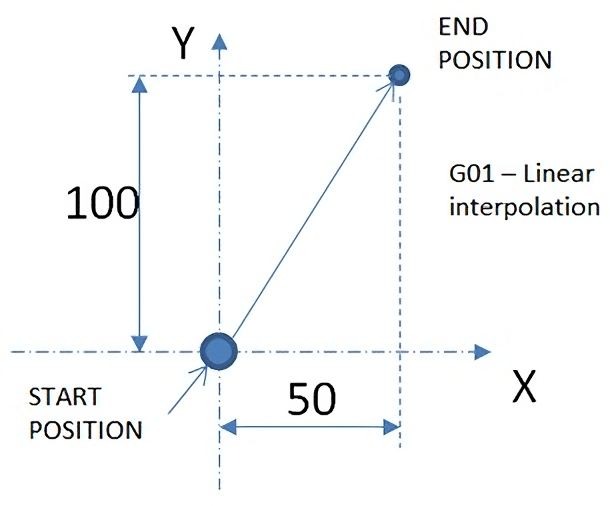
\includegraphics[width=0.5\linewidth]{imgs/g1.png}
    \caption{La instrucción: G1 X50 Y100}
    \label{g1}
\end{figure}


La instrucción G28 \textit{homing} es fundamental para establecer un punto de referencia absoluto desde el cual se medirán los movimientos de la máquina. Este proceso consiste en el desplazamiento automático del cabezal hacia los extremos de los ejes, donde se ubican los sensores de fin de carrera. Estos sensores, de naturaleza digital, detectan la llegada del cabezal y señalan que se ha alcanzado la posición límite predefinida. Una vez completado el procedimiento de homing, el sistema asigna un conjunto de coordenadas a dicha posición, comúnmente el (0,0,0), que pasa a ser el origen del sistema de coordenadas absolutas. A partir de este punto, es posible establecer orígenes relativos adicionales (G92), lo que resulta útil para optimizar ciertos procesos de fabricación, en particular aquellos que requieren operaciones repetitivas o el uso de dispositivos de montaje. Es posible hacer homing de los ejes de manera independiente, indicándolo en la instrucción (G28 X, por ejemplo).

El conjunto restante de códigos disponibles dependerá del tipo de proceso de fabricación implementado en cada máquina, así como de sus capacidades específicas y del grado de personalización definido por el fabricante. Estos códigos adicionales permiten ejecutar instrucciones complementarias, tales como el cambio automático de herramientas, el calentamiento de determinados componentes, la activación de sistemas de refrigeración, entre otras funciones necesarias para la operación del equipo.

\section{Capacidades y performance}

Uno de los parámetros más relevantes en la fabricación de una pieza es la velocidad de operación, la cual está condicionada por diferentes factores, como por ejemplo, las capacidades de los motores que componen la cadena cinemática del sistema. Si bien el objetivo suele ser minimizar el tiempo de producción aprovechando al máximo el rendimiento de los motores, un aumento en la velocidad puede generar efectos adversos. En particular, fenómenos de naturaleza mecánica, como las vibraciones o las resonancias estructurales, pueden comprometer la precisión y la calidad superficial de la pieza final.

Estos fenómenos están directamente relacionados con la construcción de la máquina y las características específicas del proceso. La rigidez global del chasis, la robustez y precisión del sistema de transmisión, la capacidad de amortiguación de la estructura, la alineación correcta entre ejes durante el ensamble, y las inercias asociadas a los componentes móviles determinan en gran medida la \textbf{respuesta dinámica del sistema}. Una estructura con baja rigidez puede experimentar deformaciones ante cargas dinámicas, mientras que transmisiones con \textbf{juego mecánico} o flexibilidad excesiva introducen errores en la trayectoria programada. Asimismo, inercias elevadas dificultan las aceleraciones controladas, y una amortiguación insuficiente puede prolongar oscilaciones no deseadas tras cambios bruscos de velocidad o dirección.


\begin{figure}[h!]
    \centering
    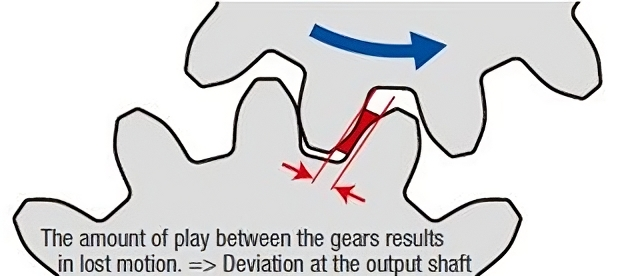
\includegraphics[width=0.7\linewidth]{imgs/gears.png}
    \caption{Juego mecánico entre dos engranajes.}
    \label{gears}
\end{figure}

El juego mecánico (backlash, en inglés) se refiere al movimiento relativo no deseado entre dos componentes mecánicos cuando se invierte la dirección del movimiento en un sistema de transmisión. Este fenómeno ocurre, por ejemplo, en engranajes, husillos, tuercas o acoplamientos, y se manifiesta como un pequeño desplazamiento libre antes de que el movimiento se transmita efectivamente. No es viable eliminar completamente el juego mecánico, es consecuencia de \textbf{tolerancias} de fabricación, desgaste o diseño intencional, y puede afectar negativamente la precisión y repetibilidad en sistemas de control numérico y máquinas de fabricación digital. Una característica positiva del juego mecánico es facilitar o hacer posible el ensamble de un sistema.

La tolerancia en un proceso de fabricación se define como la variación dimensional permitida respecto a las especificaciones nominales de una pieza, dentro de la cual el componente aún se considera funcional y conforme al diseño. Representa el rango aceptable de desviaciones en dimensiones lineales, angulares, formas o posiciones, y se establece en función de los requerimientos de ensamblaje, desempeño mecánico y costos de producción. Las tolerancias son un elemento clave en el control de calidad, ya que determinan los límites dentro de los cuales un proceso puede producir piezas sin necesidad de retrabajo o descarte. Por ejemplo, una tolerancia común en impresoras 3D de escritorio tipo FDM es de $\pm 0.5 \,\mathrm{mm}$, lo cual debe tomarse en cuenta al momento del diseño, especialmente para asegurar encajes.

Otra característica deseada en un proceso de fabricación es la precisión, nuevamente, determinada por la construcción de la máquina y el tipo de operaciones desarrolladas. En el contexto de manufactura, es importante distinguir entre \textbf{precisión} y \textbf{exactitud} (accuracy) (Figura \ref{press1}). La precisión se refiere a la consistencia de los resultados: una máquina es precisa si produce piezas con dimensiones muy similares entre sí, aunque todas estén ligeramente desviadas del valor nominal. En cambio, la exactitud indica qué tan cerca está el resultado del valor deseado o teórico. Por ejemplo, si una impresora 3D fabrica diez piezas de 20 mm y todas miden 19,7 mm, decimos que es precisa (porque es repetitiva), pero no exacta (porque hay un error sistemático).

\begin{figure}[h!]
    \centering
    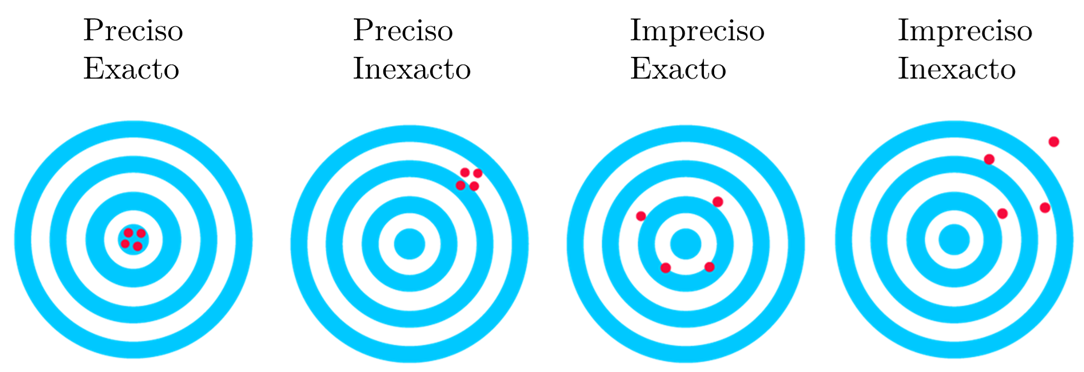
\includegraphics[width=0.9\linewidth]{imgs/press.png}
    \caption{Precisión y exactitud. La precisión se mide como la dispersión entre puntos, y la exactitud respecto al objetivo.}
    \label{press1}
\end{figure}

En una arquitectura cinemática basada en motores paso a paso, el error de exactitud está condicionado por la naturaleza discreta del paso angular. Cada pulso desplaza el eje un ángulo fijo, introduciendo un sesgo sistemático de hasta $\pm \tfrac{1}{2}$ paso o micropaso frente al valor de consigna. De este modo, ciertas posiciones teóricas resultan inalcanzables para el sistema; no obstante, la importancia de este sesgo depende de la tolerancia admitida en el proceso.

Al igual que los motores paso a paso, la instrumentación digital, a través de encoders incrementales o absolutos y convertidores analógico-digitales (ADC), introduce un error de cuantización fijo, determinado por su resolución espacial y digital: la señal analógica se discretiza en incrementos, generando un sesgo máximo de $\pm ½$ LSB (Least Significant Bit). Al mismo tiempo, el sistema de control ejecuta su loop de realimentación con una frecuencia de muestreo y actualización finitas, lo que provoca retardos equivalentes a un periodo de muestreo y variaciones de temporización (jitter) en la emisión de pulsos de actuación. Estos efectos combinados, cuantización de la instrumentación y discretización temporal del controlador, se traducen en errores sistemáticos y aleatorios de seguimiento de trayectoria, limitando la exactitud dinámica y la repetibilidad del proceso.

Finalmente,en la fase operativa de fabricación surgen múltiples fuentes de error inherentes al material y a la herramienta. Por ejemplo, el filamento de impresión 3D puede presentar variaciones de diámetro a lo largo de la bobina, además de absorber humedad o contener impurezas, lo que provoca fluctuaciones en el caudal de extrusión. Por otro lado, las herramientas de corte experimentan dilatación térmica y deflexión mecánica bajo carga y temperatura elevadas, generando desplazamientos sistemáticos en el perfil de la pieza y afectando la rugosidad de la superficie.

Así, en la fabricación por CNC, el componente real rara vez reproduce con exactitud el modelo diseñado debido a la confluencia de múltiples fuentes de imprecisión inherentes al proceso. Estas desviaciones, que emergen de la interacción entre la respuesta dinámica de la máquina, la resolución del sistema de control y la instrumentación digital y las condiciones operativas del mecanizado, deben anticiparse desde la fase de diseño geométrico y de tolerancias hasta la selección y ajuste de la máquina. De este modo, se asegura que las tolerancias dimensionales y la calidad superficial esperadas sean coherentes con el comportamiento efectivo del sistema CNC.

\section{Prototipado rápido}

En las primeras fases del desarrollo de un producto, el prototipado transforma ideas y bocetos en modelos físicos de baja fidelidad que evolucionan progresivamente hacia versiones cada vez más representativas. Este proceso culmina en un nivel de confianza suficiente para planificar la producción con seguridad. El prototipado rápido (Figura \ref{propro}) destaca como una metodología ágil al emplear máquinas de fabricación digital capaces de materializar directamente diseños CAD.

\begin{figure}[h!]
    \centering
    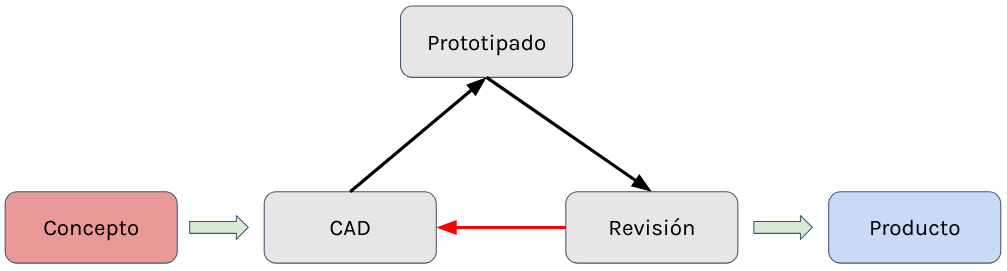
\includegraphics[width=1.0\linewidth]{imgs/prototip.png}
    \caption{Flujo de la metodología de prototipado rápido.}
    \label{propro}
\end{figure}

La visualización 3D en el CAD complementada con los módulos de análisis y simulación mecánica refuerza la confianza en la viabilidad del diseño y evita asumir prematuramente los costes de fabricación. Aunque el entorno 3D permite anteponerse incluso a obstáculos de ensamble, no puede entregar toda la información que se obtendría manipulando una maqueta o modelo a escala del producto.

Según la tecnología de fabricación digital empleada, ya sea una impresora 3D FDM de escritorio o un centro de mecanizado industrial, se pueden obtener diferentes tipos de prototipos adaptados a cada objetivo: maquetas para validar ensamblajes e interacción, piezas de alta fidelidad con acabado superficial equiparable al de un molde de inyección, o réplicas en el material definitivo para ensayos de servicio, o incluso, de manufactura.

La selección del proceso de manufactura definitiva es un paso esencial para cerrar el diseño de un producto. Aunque la fabricación digital acelera la validación de conceptos, rara vez resulta competitiva en costes al escalar a producción en serie. Sin embargo, la flexibilidad de estas tecnologías permite crear prototipos cuyas geometrías incorporan de antemano las restricciones y oportunidades de los métodos productivos finales, poniendo en práctica un enfoque de \textbf{diseño orientado a la manufactura}.